\documentclass[25pt, a0paper,
               colspace=15mm, subcolspace=0mm,
               blockverticalspace=17mm]{tikzposter} % See Section 

\usepackage{graal-poster}
\usepackage{array}
\usepackage{multirow}
\usepackage{multicol}


\definecolor{PaleBlue}{rgb}{0,.55,.9}
\definecolor{PaleGreen}{rgb}{0,.7,.25}
\definecolor{RedPink}{rgb}{.9,0,.2}
\definecolor{Pink}{rgb}{.85,.35,.7}
\definecolor{Purple}{rgb}{.6,0,.75}
\definecolor{Orange}{rgb}{.9,.3,.05}

\colorlet{attentionColor}{Orange}
\colorlet{charEmbedColor}{RedPink}
\colorlet{predEmbedColor}{Pink}
% \colorlet{attentionColor}{GoldUL!90!black}
% \definecolor{attentionColor}{rgb}{.85,.5,.6}



\def\pathwidth{2pt}
\def\nodewidth{3pt}
\def\cornerCurvature{7pt}

\tikzstyle{embed}=[%
  draw,
  #1,
  % line width=3pt,
  anchor=north,
  minimum width=.8cm,
  minimum height=1.6cm,
  inner sep=0pt,
  text=#1!65!black,
  font=\fontsize{25pt}{24}\selectfont,
  ]




\title{\parbox{\linewidth}{\centering Leveraging Subword Embeddings for Multinational Address Parsing}}
\institute{Department of Computer Science and Software Engineering, Université Laval}
\author{Marouane Yassine, David Beauchemin, François Laviolette, Luc Lamontagne}

\begin{document}
\maketitle

\begin{columns}
\column{.4}
\block{Introduction}{%
We propose an approach in which we employ subword embeddings and a Recurrent Neural Network (RNN) architecture to build a single model capable of learning to parse addresses from multiple countries at the same time while taking into account the difference in languages and address formatting systems.

\vspace{5mm}
\textbf{Motivations:}
\begin{itemize}
  \item Address parsing is an essential part of many applications, such as geocoding and record linkage.
  \item The only multinational solution takes a heavy pre-preprocessing and post-preprocessing step and a considerable amount of meta-data.
\end{itemize}

\vspace{5mm}
\textbf{Related work:}
\begin{itemize}
  \item Sharma et al. (2018): Parse monolingual address using a feedforward neural network.
  \item Mokhtari et al. (2019): Parse monolingual address using different RNN architectures.
\end{itemize}

\vspace{0mm}
\textbf{Goals:}
\begin{itemize}
  \item Provide multinational address parsing using a single model.
  \item Provide a more meaningful way to handle OOV words using subword embeddings.
  \item Evaluate the degree to which a model trained on countries' addresses data can perform well at parsing addresses from other countries (zero shot evaluation).
\end{itemize}

% \vspace{-15pt}

}

\column{0.6}
\block{Subword Embeddings}{

\vspace{-15pt}
% Comick v3.0 (TheFinalComick)

\textbf{Word embedding} : vector representation of a word
\begin{itemize}
    \item Non-contextual embeddings (e.g : Word2Vec, Glove)
    \item Contextual embeddings (e.g : ELMo, BERT)
\end{itemize}

\textbf{Subword embedding} : vector representation of a unit
\begin{itemize}
    \item Character level
    \item Character n-grams (e.g : the bi-gram of "H1A 1B1" is {H1, 1A,
A1, 1B, B1}) (e.g : fastText)
    \item Byte pair embeddings (e.g: the byte pair of "H1A 1B1" is \{\_H, 0, a, 0, b, 0\}) (e.g: \textit{BPEmb})
\end{itemize}

}

\block{Architecture}{
\textbf{Embedding model} : We compare two pre-trained embedding
\begin{itemize}
    \item A fixed pre-trained monolingual fastText model (pre-trained on the French language) (\textbf{fastText}).
    \item A encoding of words using MultiBPEmb and merge the obtained embeddings for each word into one word embedding using a Bidirectional LSTM (Bi-LSTM) (hidden state dimension of $300$) (\textbf{BPEmb}).
\end{itemize}

\textbf{Tagging model} : We use a Seq2Seq model consisting of
		\begin{itemize}
			\item a one-layer unidirectional LSTM encoder
			\item a one-layer unidirectional LSTM decoder
			\item a fully-connected linear layer to map the representation into the tag space dimensionality (i.e. the number of tags)
			\item a softmax activation. 
		\end{itemize}

}
\end{columns}

\begin{columns}


  \column{.4}
  \block{Data}{
        \begin{itemize}
			\item Built using the open-source data of Libpostal.
			\item Contain $61$ countries.
			\item We used eight tags: StreetNumber, StreetName, Unit, Municipality, Province, PostalCode, Orientation, and GeneralDelivery.
		\end{itemize}
	We use five different address patterns (one for each color) and some countries use more than one of these patterns (no color). The following figure presents three of them.

	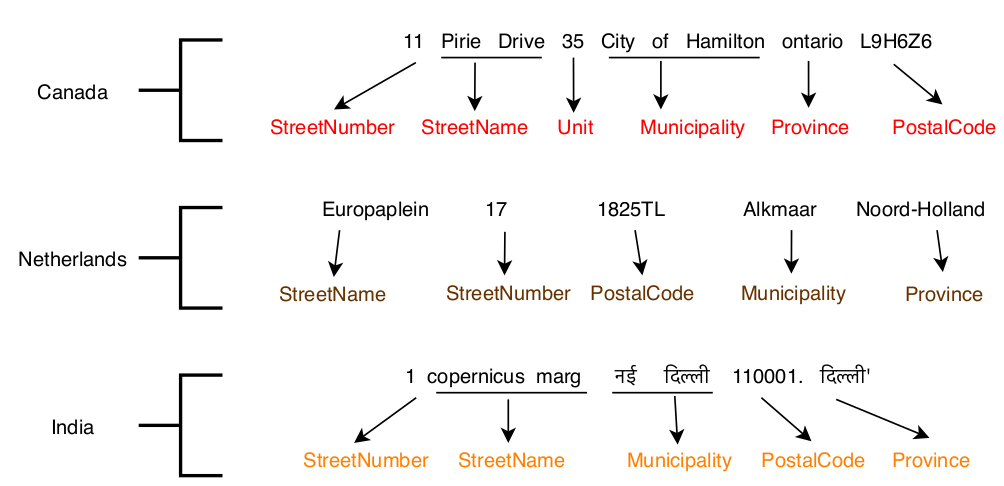
\includegraphics[width=0.3\textwidth,height=0.25\textheight,keepaspectratio]{figures/Samples2.png}


  }
  
    \column{.6}
  \block{Experiments}{
  \textbf{Training data:}
  \begin{itemize}
      \item $20$ countries are used for multinational training with a sample size of $100,000$ per country. The rest is used as a holdout.
      \item $41$ countries are used for zero-shot transfer evaluation (never seen in training).
  \end{itemize}
    \textbf{Training procedure:}
    \begin{itemize}
			\item We trained each of our two models five times\footnote{With the following seed $\{5, 10, 15, 20, 25\}$.}  (\textbf{fastText} and \textbf{BPEmb}).
			\item They were trained during $200$ epochs with a batch size of $2048$.
			\item We used an early stopping with a patience of 15 epochs.
			\item A starting learning rate at $0.1$ and a learning rate scheduling (factor of $0.1$) after ten epochs without loss decrease. 
			\item Cross-Entropy loss.
			\item Stochastic Gradient Descent (SGD) optimizer.
			\item Teacher forcing.
			\item Trained using Poutyne.
		\end{itemize}


  }




\end{columns}





\begin{columns}

  \column{.28}


  \block{Multinational Evaluation}{

  \resizebox{0.24\textwidth}{!}{%
			\begin{tabular}{cccccc}
				\toprule
				Country & \textbf{FastText} & \textbf{BPEmb} & Country & \textbf{FastText} & \textbf{BPEmb}\\
				\midrule
				United States & $\mathbf{99.61 \pm 0.09}$ & $98.55 \pm 2.19$ & Poland & $\mathbf{99.69 \pm 0.07}$ & $99.19 \pm 1.39$\\
				Brazil & $\mathbf{99.40 \pm 0.10}$ & $98.54 \pm 1.68$ & Norway & $\mathbf{99.46 \pm 0.06}$ & $97.98 \pm 1.31$\\
				South Korea & $99.96 \pm 0.01$ & $\mathbf{99.99 \pm 0.02}$ & Austria & $\mathbf{99.28 \pm 0.03}$ & $98.28 \pm 1.56$\\
				Australia & $\mathbf{99.68 \pm 0.05}$ & $99.21 \pm 1.17$ & Finland & $\mathbf{99.77 \pm 0.03}$ & $99.72 \pm 0.30$\\
				Mexico & $\mathbf{99.60 \pm 0.06}$ & $98.55 \pm 2.22$ & Denmark & $\mathbf{99.71 \pm 0.07}$ & $99.20 \pm 1.38$\\
				Germany & $\mathbf{99.77 \pm 0.04}$ & $99.23 \pm 1.30$ & Czechia & $\mathbf{99.57 \pm 0.09}$ & $98.77 \pm 2.22$\\
				Spain & $\mathbf{99.75 \pm 0.05}$ & $98.65 \pm 2.36$ & Italy & $\mathbf{99.73 \pm 0.05}$ & $98.91 \pm 1.76$\\
				Netherlands & $\mathbf{99.61 \pm 0.07}$ & $99.26 \pm 1.23$ & France & $\mathbf{99.66 \pm 0.08}$ & $98.65 \pm 2.00$\\
				Canada & $\mathbf{99.79 \pm 0.05}$ & $99.19 \pm 1.33$ & United Kingdom & $\mathbf{99.61 \pm 0.10}$ & $98.66 \pm 2.11$\\
				Switzerland & $\mathbf{99.53 \pm 0.09}$ & $99.49 \pm 0.53$ & Russia & $\mathbf{99.03 \pm 0.24}$ & $97.52 \pm 4.23$\\
				\bottomrule
			\end{tabular}%
		}

	\begin{itemize}
	    \item \textbf{FastText} gives the best performance across the board without considering the standard deviation.
	    \item South Korean results are excellent despite the completely different alphabet.
	    \item When using standard deviation, the \textbf{BPEmb} model achieves better results than \textbf{fastText} in most cases.
		\item We find that South Korea is the only country where a perfect accuracy ($100~\%$) was achieved using \textbf{BPEmb} ($3$ out of $5$). 
		\item Randomly reordering $6000$ South Korean addresses as either the first (red) or the second (brown) address pattern (equally divided between the two), the mean accuracy drops to $28.04\%$ (the mean accuracy is of $12.29~\%$ using a random tags procedure).
	\end{itemize}


  }
  
    \column{.38}


  \block{Zero-shot Evaluation}{

  \resizebox{0.34\textwidth}{!}{%
		\begin{tabular}{cccccc}
				\toprule
				Country & \textbf{FastText} & \textbf{BPEmb} & Country & \textbf{FastText} & \textbf{BPEmb}\\
				\midrule
				Belgium & $\mathbf{88.14 \pm 1.04}$ & $87.45 \pm 1.37$ & Faroe Islands & $74.14 \pm 1.83$ & $\mathbf{86.59 \pm 2.21}$\\
				Sweden & $81.59 \pm 4.53$ & $\mathbf{88.30 \pm 2.92}$ & Réunion & $\mathbf{96.80 \pm 0.45}$ & $92.42 \pm 2.38$\\
				Argentina & $\mathbf{86.26 \pm 0.47}$ & $86.00 \pm 4.40$ & Moldova & $\mathbf{90.18 \pm 0.79}$ & $78.11 \pm 16.79$\\
				India & $69.09 \pm 1.74$ & $\mathbf{76.33 \pm 7.77}$ & Indonesia & $64.31 \pm 0.84$ & $\mathbf{69.25 \pm 2.81}$\\
				Romania & $\mathbf{94.49 \pm 1.52}$ & $90.52 \pm 2.35$ & Bermuda & $92.31 \pm 0.60$ & $\mathbf{92.65 \pm 1.84}$\\
				Slovakia & $82.10 \pm 0.98$ & $\mathbf{89.40 \pm 5.09}$ & Malaysia & $78.93 \pm 3.78$ & $\mathbf{92.76 \pm 2.55}$\\
				Hungary & $\mathbf{48.92 \pm 3.59}$ & $24.61 \pm 3.35$ & South Africa & $\mathbf{95.31 \pm 1.68}$ & $92.75 \pm 7.43$\\
				Japan & $\mathbf{41.41 \pm 3.21}$ & $33.34 \pm 3.83$ & Latvia & $\mathbf{93.66 \pm 0.64}$ & $72.46 \pm 5.77$\\
				Iceland & $96.55 \pm 1.20$ & $\mathbf{97.61 \pm 0.98}$ & Kazakhstan & $86.33 \pm 3.06$ & $\mathbf{88.28 \pm 11.32}$\\
				Venezuala & $\mathbf{94.87 \pm 0.53}$ & $89.82 \pm 5.74$ & New Caledonia & $\mathbf{99.48 \pm 0.15}$ & $96.44 \pm 5.64$\\
				Philippines & $77.76 \pm 3.97$ & $\mathbf{78.00 \pm 11.75}$ & Estonia & $\mathbf{87.08 \pm 1.89}$ & $76.18 \pm 1.62$\\
				Slovenia & $95.37 \pm 0.23$ & $\mathbf{96.47 \pm 2.05}$ & Singapore & $\mathbf{86.42 \pm 2.36}$ & $83.23 \pm 6.38$\\
				Ukraine & $\mathbf{92.99 \pm 0.70}$ & $90.86 \pm 2.90$ & Bangladesh & $78.61 \pm 0.43$ & $\mathbf{79.77 \pm 3.65}$\\
				Belarus & $\mathbf{91.08 \pm 3.08}$ & $90.16 \pm 11.89$ & Paraguay & $96.01 \pm 1.23$ & $\mathbf{96.22 \pm 1.78}$\\
				Serbia & $\mathbf{95.31 \pm 0.48}$ & $88.49 \pm 7.05$ & Cyprus & $\mathbf{97.67 \pm 0.34}$ & $92.92 \pm 6.94$\\
				Croatia & $\mathbf{94.59 \pm 2.21}$ & $88.17 \pm 4.58$ & Bosnia & $\mathbf{84.04 \pm 1.47}$ & $80.53 \pm 6.56$\\
				Greece & $\mathbf{81.98 \pm 0.60}$ & $35.30 \pm 13.51$ & Ireland & $\mathbf{87.44 \pm 0.69}$ & $84.93 \pm 2.85$\\
				New Zealand & $94.27 \pm 1.50$ & $\mathbf{97.77 \pm 3.23}$ & Algeria & $\mathbf{85.37 \pm 2.05}$ & $79.66 \pm 11.68$\\
				Portugal & $\mathbf{93.65 \pm 0.46}$ & $90.13 \pm 4.47$ & Colombia & $\mathbf{87.81 \pm 0.92}$ & $87.60 \pm 3.61$\\
				Bulgaria & $\mathbf{91.03 \pm 2.07}$ & $87.44 \pm 11.94$ & Uzbekistan & $\mathbf{86.76 \pm 1.13}$ & $73.75 \pm 3.42$\\
				Lithuania & $\mathbf{87.67 \pm 3.05}$ & $75.67 \pm 2.19$ &  &  & \\
				\bottomrule
			\end{tabular}%
		}
    \begin{itemize}
			\item $50~\%$ ($19$ out of $41$) near state-of-the-art performance ($>90~\%$) for \textbf{fastText}. Or $35~\%$ for \textbf{BPEmb}.
			\item $80~\%$ ($34$ out of $41$) good performance ($>80~\%$) for \textbf{fastText}. Or $65~\%$ for \textbf{BPEmb}.
			\item The lowest results (below $70\%$) occur for countries where the address pattern and the country official language were not seen in the training data such as India, Hungary, and Japan. 
	\end{itemize}
  }


  
  
  \column{.34}
  
    \block{Zero-shot Evaluation Discussion}{
    For Hungary and Japan, the poorest results are mostly due to the address structure (blue), which is the near inverse of the two most present ones (red and brown) (never seen structure and language).
    
    Kazakhstan, which uses the same address pattern as Japan, achieves better results. The main difference being the presence of one of the official language (Kazakh and \textbf{Russian}) in the training dataset.
    
    India achieves almost $20\%$ better results than Hungary and Japan, even if Hindi does not occur in the training dataset. Due to the use of a nearly identical address pattern as the first one (red). The only difference being the inversion of the province and the postal code.
  }
  \block{Conclusion}{
    \begin{itemize}
        \item Tackled the multinational address parsing problem with SOTA results.
		\item We explored the possibility of zero-shot transfer across countries.
    \end{itemize}
    
    \textbf{Future Work:}
    \begin{itemize}
        \item  Attention mechanism
        \item Domain-adversarial training techniques (e.g. DANN or ADANN)
    \end{itemize}
  }
\end{columns}

\end{document}
